\documentclass[tikz,border=10pt]{standalone}
\usepackage[T1]{fontenc}
\usepackage{lmodern}
\usetikzlibrary{arrows.meta, calc}

\definecolor{human}{HTML}{4477AA}
\definecolor{ai}{HTML}{228833}
\definecolor{arrcol}{HTML}{444444}
\definecolor{labelcol}{HTML}{666666}
\definecolor{cyclecol}{HTML}{666666}
\definecolor{annotcol}{HTML}{888888}
\definecolor{warncol}{HTML}{CC3311}
\definecolor{memcol}{HTML}{886644}
\definecolor{revcol}{HTML}{884488}

\begin{document}
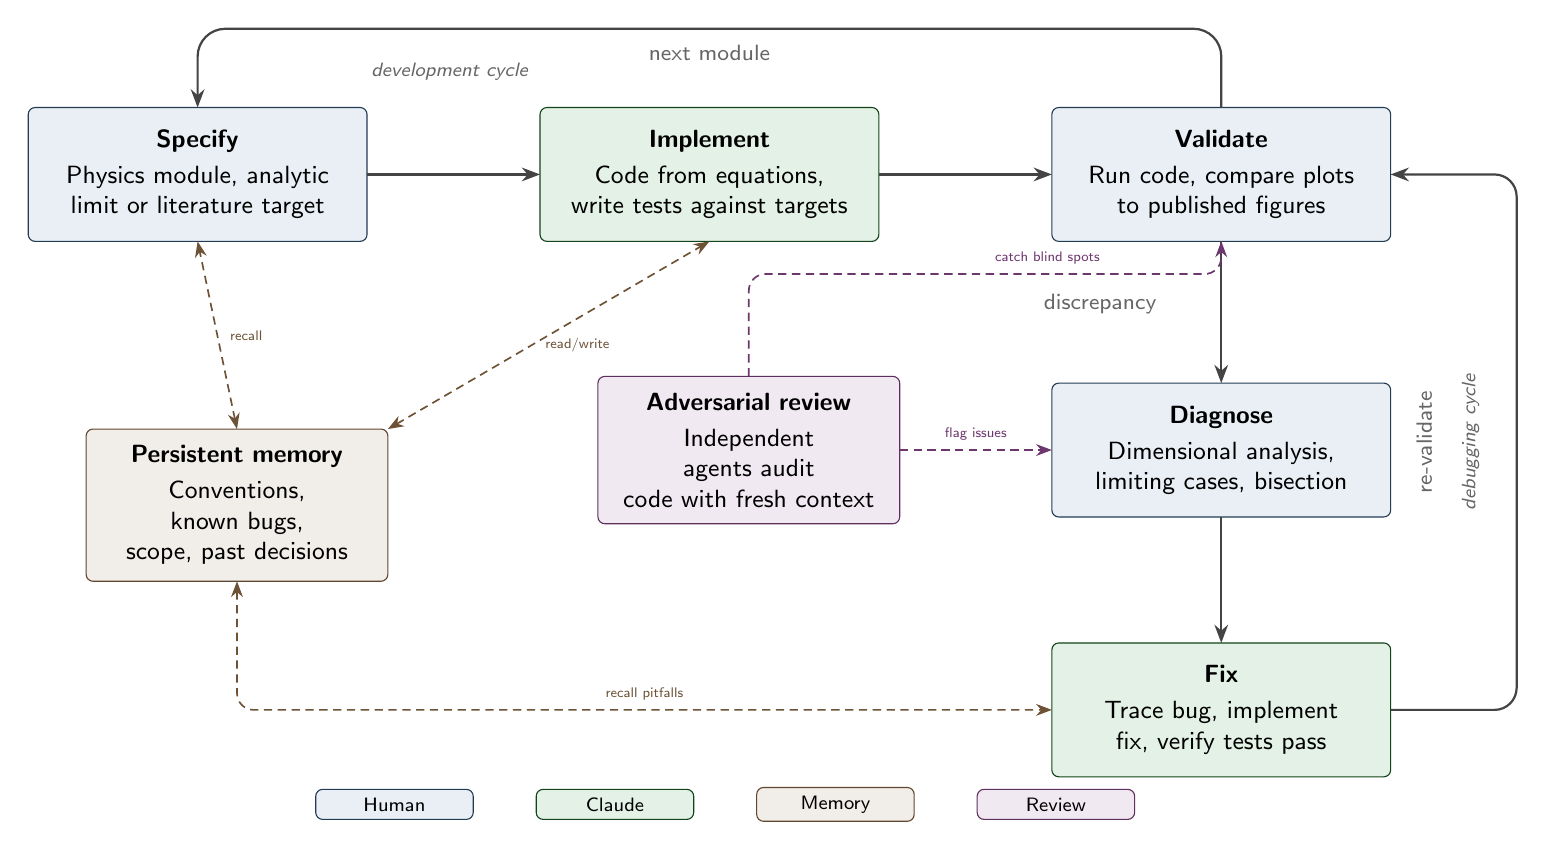
\begin{tikzpicture}[
    >=Stealth,
    every node/.style={font=\sffamily},
    hbox/.style={
        draw=human!50!black, fill=human!12, rounded corners=2.5pt,
        align=center, font=\sffamily\small, line width=0.4pt,
        inner xsep=10pt, inner ysep=7pt, text width=3.6cm, minimum height=1.7cm,
        outer sep=0pt,
    },
    abox/.style={
        draw=ai!50!black, fill=ai!12, rounded corners=2.5pt,
        align=center, font=\sffamily\small, line width=0.4pt,
        inner xsep=10pt, inner ysep=7pt, text width=3.6cm, minimum height=1.7cm,
        outer sep=0pt,
    },
    membox/.style={
        draw=memcol!70!black, fill=memcol!12, rounded corners=2.5pt,
        align=center, font=\sffamily\small, line width=0.4pt,
        inner xsep=9pt, inner ysep=6pt, text width=3.2cm, minimum height=1.5cm,
        outer sep=0pt,
    },
    revbox/.style={
        draw=revcol!70!black, fill=revcol!12, rounded corners=2.5pt,
        align=center, font=\sffamily\small, line width=0.4pt,
        inner xsep=9pt, inner ysep=6pt, text width=3.2cm, minimum height=1.5cm,
        outer sep=0pt,
    },
    arr/.style={->, line width=0.8pt, draw=arrcol},
    memarr/.style={<->, line width=0.6pt, draw=memcol!80!black, densely dashed},
    revarr/.style={->, line width=0.6pt, draw=revcol!80!black, densely dashed},
    lbl/.style={font=\sffamily\footnotesize, text=labelcol},
    annot/.style={font=\sffamily\tiny\itshape, text=annotcol},
    warn/.style={font=\sffamily\tiny, text=warncol},
]

% === Main chain (top row) ===
\node[hbox] (spec) at (0, 0) {
    \textbf{Specify}\\[2pt]
    Physics module, analytic\\limit or literature target
};
\node[abox] (impl) at (6.5, 0) {
    \textbf{Implement}\\[2pt]
    Code from equations,\\write tests against targets
};
\node[hbox] (val) at (13, 0) {
    \textbf{Validate}\\[2pt]
    Run code, compare plots\\to published figures
};

% === Debugging loop (right column) ===
\node[hbox] (diag) at (13, -3.5) {
    \textbf{Diagnose}\\[2pt]
    Dimensional analysis,\\limiting cases, bisection
};
\node[abox] (fix) at (13, -6.8) {
    \textbf{Fix}\\[2pt]
    Trace bug, implement\\fix, verify tests pass
};

% === Supporting elements ===
\node[membox] (memory) at (0.5, -4.2) {
    \textbf{Persistent memory}\\[2pt]
    Conventions, known bugs,\\scope, past decisions
};
\node[revbox] (review) at (7, -3.5) {
    \textbf{Adversarial review}\\[2pt]
    Independent agents audit\\code with fresh context
};

% === Main flow arrows ===
\draw[arr] (spec) -- (impl);
\draw[arr] (impl) -- (val);

% Outer loop: Validate -> Specify (over top)
\draw[arr, rounded corners=10pt]
    (val.north) -- ++(0, 1.0) -| (spec.north);
\node[lbl] at (6.5, 1.55) {next module};
\node[font=\sffamily\scriptsize\itshape, text=cyclecol] at (3.2, 1.3) {development cycle};

% Validate -> Diagnose (down)
\draw[arr] (val.south) -- (diag.north);
\node[lbl, anchor=east] at (12.3, -1.65) {discrepancy};

% Diagnose -> Fix (down)
\draw[arr] (diag.south) -- (fix.north);

% Fix -> Validate (loop back, right side)
\draw[arr, rounded corners=8pt]
    (fix.east) -- ++(1.6, 0) |- (val.east);
\node[lbl, rotate=90, anchor=south] at (15.8, -3.4) {re-validate};
\node[font=\sffamily\scriptsize\itshape, text=cyclecol, rotate=90, anchor=south]
    at (16.4, -3.4) {debugging cycle};

% === Memory connections ===
% Memory <-> Specify (straight up, clean)
\draw[memarr] (memory.north) -- (spec.south)
    node[midway, right, font=\sffamily\tiny, text=memcol!80!black, xshift=1pt] {recall};

% Memory <-> Implement (clean diagonal, avoids annotation area)
\draw[memarr, rounded corners=5pt]
    (memory.north east) -- (impl.south)
    node[pos=0.45, right, font=\sffamily\tiny, text=memcol!80!black, xshift=1pt] {read/write};

% Memory <-> Fix (from memory bottom, right along bottom, up to fix)
\draw[memarr, rounded corners=6pt]
    (memory.south) |- (fix.west)
    node[pos=0.75, above, font=\sffamily\tiny, text=memcol!80!black] {recall pitfalls};

% === Adversarial review connections ===
% Review -> Diagnose (horizontal, same y-level — clean)
\draw[revarr] (review.east) -- (diag.west)
    node[midway, above, font=\sffamily\tiny, text=revcol!80!black] {flag issues};

% Review -> Validate (routed above review, right-angle to avoid annotation zone)
\draw[revarr, rounded corners=6pt]
    (review.north) -- ++(0, 1.3) -| (val.south)
    node[pos=0.25, above right, font=\sffamily\tiny, text=revcol!80!black] {catch blind spots};


% === Legend (centered under figure) ===
\node[hbox, text width=1.2cm, minimum height=0cm, minimum width=2.0cm,
      inner ysep=3pt, inner xsep=5pt, font=\sffamily\scriptsize] at (2.5, -8.0) {Human};
\node[abox, text width=1.2cm, minimum height=0cm, minimum width=2.0cm,
      inner ysep=3pt, inner xsep=5pt, font=\sffamily\scriptsize] at (5.3, -8.0) {Claude};
\node[membox, text width=1.2cm, minimum height=0cm, minimum width=2.0cm,
      inner ysep=3pt, inner xsep=5pt, font=\sffamily\scriptsize] at (8.1, -8.0) {Memory};
\node[revbox, text width=1.2cm, minimum height=0cm, minimum width=2.0cm,
      inner ysep=3pt, inner xsep=5pt, font=\sffamily\scriptsize] at (10.9, -8.0) {Review};

\end{tikzpicture}
\end{document}
